\chapter{Safety and Security Properties}\label{sec:defsafetyissues}

While the model evaluation methods in Chapter~\ref{sec:usualevaluation} can provide certain insights into the quality of machine learning models, their evaluations  completely rely on the training and test datasets, without considering other factors that might potentially compromise the performance of a machine learning model. Actually, safety risks may appear at any stage of the lifecycle 
%(including mainly three stages: data collection and preparation, model construction and training, and model deployment and operational use) 
of a machine learning model. In recent years, the discussion on the potential risks of machine learning models has been very intense, and many risks have been discovered, even though the models have achieved excellent performance with respect to the traditional model evaluation methods. This chapter will discuss a set of safety and security properties. 

%The second set of evaluation methods are more involved, and are intensively studied in recent years.  
%
%Despite the success of machine learning in many areas, serious concerns have been raised in applying machine learning to real-world safety-critical systems such as self-driving cars, automatic medical diagnosis, etc.
%So, the second group of evaluation methods focuses on a few safety and reliability issues of machine learning.
%that we will explore in the next sections. 


Simply speaking, a learned model $f$ is to approximate a target function $h$. Therefore, the erroneous behaviour of $f$ exists when it is inconsistent with $h$. We use 
 $f_j(\textbf{x})$ to denote its $j$-th element of $f(\textbf{x})$. Then, we have the following definition for the classification task.  
%Moreover, for simplicity, let $n=s_1$ be the number of input dimensions and $m=s_K$ be the number of output dimensions. 


\begin{definition}[Erroneous Behavior of a Classifier]
Given a (trained) classifier $f: \real^{n} \to \real^{k}$, a target function $\humanoracle: \real^{n} \to \real^{k}$, an erroneous behavior of the classifier $f$ is exhibited by a legitimate input $\textbf{x}\in \real^{n}$ such that 
\begin{equation}
\argmax_j f_j(\textbf{x}) \neq \argmax_j \humanoracle_j(\textbf{x})
\end{equation}
\end{definition}
%
Intuitively, an erroneous behaviour is witnessed by the existence of an input $\textbf{x}$ on which the classifier and the target function return a different label. Note that, the legitimate input $\textbf{x}$ can be any input in the input domain $\real^{n}$ and does not have to be a training instance. 

In the following, we discuss several classes of  properties that might affect the safe use of machine learning models in real-world safety-critical applications. 




\section{Generalisation Error}\label{sec:generalisationerror}

One of the key successes of machine learning is that it is able to work with unseen data, i.e., data instances that are not within the training dataset. It is meaningful to understand how good a model is on unseen data. Given an instance $\textbf{x}$, we use a loss function to measure the discrepancy between the true label $y$ and the model's predicted label $f(\textbf{x})$, written as ${\cal L}(y, f(\textbf{x}))$. 

Given a training dataset $D_{train}$ sampled i.i.d. from the underlying distribution ${\cal D}$, the model $f$'s empirical loss on $D_{train}$, or train loss, is 
\begin{equation}
    {\cal L}_{emp}(f,D_{train}) ≝ \frac{1}{|D_{train}|}\sum_{(\textbf{x},y)\in D_{train}}{\cal L}(y, f(\textbf{x}))
\end{equation}
while the expected loss is 
\begin{equation}\label{equ:generalisationlossfunc}
    {\cal L}_{exp}(f,{\cal D}) ≝ \mathbb{E}_{(\textbf{x},y)\in {\cal D}}{\cal L}(y, f(\textbf{x}))
\end{equation}
Their gap 
\begin{equation}
    GE(f,D_{train},\mathcal{D}) = |{\cal L}_{emp}(f,D_{train}) - {\cal L}_{exp}(f,\mathcal{D})|
\end{equation}
is called generalisation error. 
The empirical test loss 
\begin{equation}
    {\cal L}_{emp}(f,D_{test}) ≝ \frac{1}{|D_{test}|}\sum_{(\textbf{x},y)\in D_{test}}{\cal L}(y, f(\textbf{x}))
\end{equation}
is often used to approximate the expected loss ${\cal L}_{exp}(f,{\cal D})$, since the underlying distribution
${\cal D}$ is unknown to the learning algorithm. Therefore, $GE(f,D_{train},\mathcal{D})$ can be approximated with 
\begin{equation}
    GE(f,D_{train},D_{test}) = |{\cal L}_{emp}(f,D_{train}) - {\cal L}_{emp}(f,D_{test})|
\end{equation}
Recall that, the test error $Err(f,D_{test})$ (Equation (\ref{equ:testerror})) is an empirical test loss when the loss function ${\cal L}$ is the 0-1 loss.
%and the dataset $D$ is the test dataset. 

Generalisation error is related to the well-known overfitting problem of machine learning algorithms. A machine learning model is overfitted if it performs  well on training data instances but badly on test data instances. Usually, a large generalisation error indicates overfitting. Moreover, generalisation error is also related to the representativeness of training and test datasets. For a high-dimensional problem, if the training and test datasets do not contain a sufficiently large amount of data instances, the estimated generalisation error will not be accurate. An inaccurate estimation will lead to a bad judgement on the quality of the machine learning model over future inputs and may lead to safety implications. 

As will be discussed in Chapter~\ref{chap:generalisationPAC}, there are other factors that may affect the generalisation ability of machine learning models, including e.g., the hyper-parameters, the model structure, and the learnable parameters. 


\section{Uncertainty}\label{sec:uncertainty}

Machine learning can be seen as an approach of implementing inductive reasoning, because it generalises from a set of observations and obtains a model that can serve as a general principle. However, a learned model will not be provably correct -- as discussed in Section~\ref{sec:generalisationerror} and Chapter~\ref{sec:usualevaluation}, a trained model $f$ may output incorrect decisions. Uncertainty quantification in machine learning is to quantitatively measure the uncertainty in the decisions made by a machine learning model. 

Other than the inherent uncertainty from the above-mentioned inductive inference, considering the development process of machine learning, there are other uncertainties such as the incorrect model assumption, nonoptimal hyper-parameters, and noisy and imprecise data. A solid representation of uncertainty may contribute well to the trustworthiness of AI, as discussed in Section~\ref{sec:assuredPartnership}.  

There are two inherently different sources of uncertainty: aleatoric and epistemic uncertainty. \emph{Aleatoric uncertainty} refers to the variability in the outcome of an experiment due to an inherently random effect. For example, in a coin-flipping experiment, the outcome of the experiment is inherently random. The inherent stochastic nature suggests that aleatoric uncertainty cannot be reduced even with the optimal model. On the other hand, \emph{epistemic uncertainty} refers to the lack of knowledge. The decision-maker may not have the full information about the problem due to the ignorance.  For example, on seeing the observations 0,0,1 of a series of coin-flipping experiments, it is unclear whether we should model the coin as a fair one or not. As opposed to the aleatoric uncertainty, epistemic uncertainty can be reduced or eliminated if provided with sufficient information, such as infinite observations in the coin-flipping experiments. In other words, we may roughly refer aleatoric uncertainty as the irreducible part of the total uncertainty and epistemic uncertainty as the reducible part of the total uncertainty.  

\subsection*{Sources of Uncertainty for Classification}

First of all, the classification problem $f(\textbf{x})$ is actually to find a conditional probability $p(y|\textbf{x})$, which returns a probability value for every class $y\in C$ when observing an instance $\textbf{x}$. However, due to the above-mentioned uncertainties, such a conditional probability is not fixed, i.e., there may be multiple, or even infinite, probabilities $p(y|\textbf{x})$ when given $\textbf{x}$. Based on this, we can have a Bayes predictor $h^*$ that computes  
\begin{equation}
    h^*(\textbf{x}) \defequal \argmin_{\hat{y}}\int_{y}\mathcal{L}(y,\hat{y})dp(y|\textbf{x})
\end{equation}
for every input instance $\textbf{x}$. We can see that, the Bayes predictor $h^*$ considers all possibilities of $p(y|\textbf{x})$ and intends to get the best prediction on average. We remark that, the uncertainty in $p(y|\textbf{x})$ is aleatoric uncertainty, as it is inherently random. 

Moreover, given a hypothesis class $\mathcal{H}$ and Equation (\ref{equ:generalisationlossfunc}), we may find the best classifier among $\mathcal{H}$, i.e., 
\begin{equation}
    f^* \defequal \argmin_{f\in \mathcal{H}} \mathcal{L}_{exp}(f,\mathcal{D})
\end{equation}
The gap between $f^*$ and $h^*$ is from the uncertainty about the right type of model to construct and fit. We call such uncertainty as \emph{model uncertainty}. 

Finally, training algorithms are locally optimal, instead of globally optimal, which means that we may not be able to achieve $f^*$ in the end, but rather a model $\hat{f}$. The gap between $\hat{f}$ and $f^*$ is from an uncertainty we call \emph{approximation uncertainty}. 

Both model uncertainty and approximation uncertainty are epistemic uncertainty, because they are  due to the lack of knowledge and can -- in theory -- be reduced. Also, the above three uncertainties (uncertainty in $p(y|\textbf{x})$, model uncertainty, approximation uncertainty) correspond to the three errors (Bayes error, model error, approximation error) to be discussed in Section~\ref{sec:archNtraining}. 


\iffalse 

\subsection*{A Decision Problem}


Take a Bayesian view on the problem and assume that we have a model parameterised with a set $\textbf{W}$ of parameters. We have $P(\textbf{W}~|~D_{train})$ as a posterior distribution, and $P(y~|~\textbf{x},\textbf{W})$ a conditional probability predicting the label according to the model parameter $\textbf{W}$ and the input $\textbf{x}$. 
   A decision problem for the uncertainty over a given instance $(\textbf{x},y)$ is to determine  if the variance of $P(y~|~\textbf{x},\textbf{W}) P(\textbf{W}~|~D_{train})$ is greater than $\sigma$, 
   %\begin{equation}
%       \int P(y~|~\textbf{x},\textbf{W}) P(\textbf{W}~|~D_{train})d\textbf{W} > \sigma
%   \end{equation}
   for $\sigma>0$ is an acceptable level of confidence. That is, it is an expected prediction probability of  $P(y~|~\textbf{x},\textbf{W})$, weighted over the posterior distribution $P(\textbf{W}~|~D_{train})$. 

\fi

\section{Robustness and Adversarial Examples}\label{sec:adversarialexample}



%Erroneous behaviours include those training and test samples which are classified incorrectly by the model and have safety implications. 
Adversarial examples \cite{szegedy2014intriguing} represent another class of erroneous behaviours that also introduce safety implications. Here, we take the name ``adversarial example'' due to historical reasons. Actually, as suggested in the below definition, it represents a mis-match of the decisions made by a human and by a machine learning model, and does not necessarily involve an adversary.  

Intuitively, as shown in Figure~\ref{fig:safetytrafficlight}, it is possible that, given an instance $\textbf{x}$, it is classified correctly, i.e., $y=\hat{f}(\textbf{x})$, but a small perturbation on $\textbf{x}$ (such as the one-pixel change as in Figure~\ref{fig:safetytrafficlight}) may lead to a change of classification, i.e., $\hat{f}(\textbf{x}+\epsilon)\neq \hat{f}(\textbf{x})$. Such misclassification may have serious security implications, as the traffic light example in Figure~\ref{fig:safetytrafficlight}. 

\begin{figure}[!thbp]
  \centering
  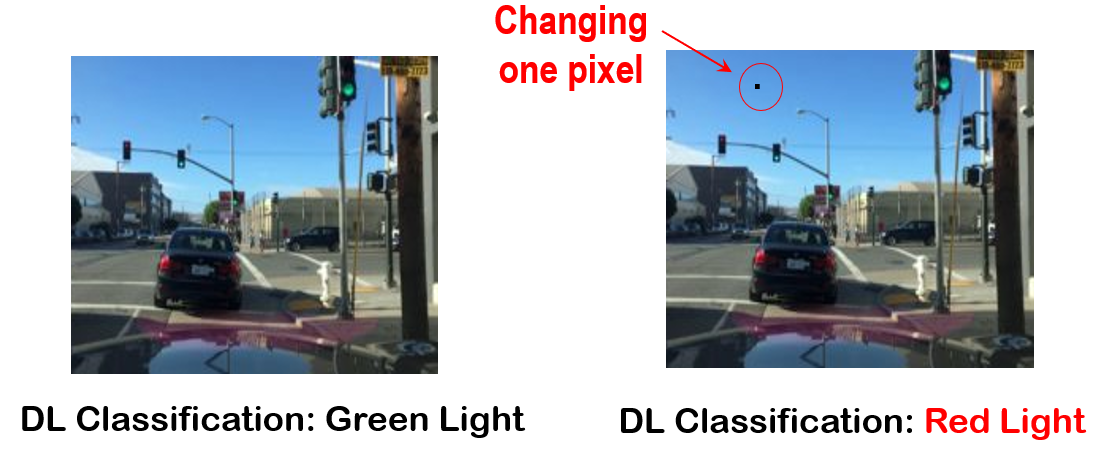
\includegraphics[width=0.8\linewidth]{images/safetyIssues/intro9.png}
  \caption{By changing one pixel in a ``Green-Light'' image, a state-of-the-art deep learning (DL) image classifier misclassifies it as ``Red-Light'' \cite{wu2018game}}
  \label{fig:safetytrafficlight}
\end{figure}

For the \textbf{iris} dataset, if we create a new data instance, indexed as 151 in the below Table~\ref{tab:irisdatasetadv}, such that the only difference with the one indexed as 150 is the petal width, from 1.8 to 1.6. A well trained decision tree classifier may  classify the new instance  as a different class.  
\begin{table}[!htbp]
\center
\small
\begin{minipage}{0.3\textwidth}
    \centering
    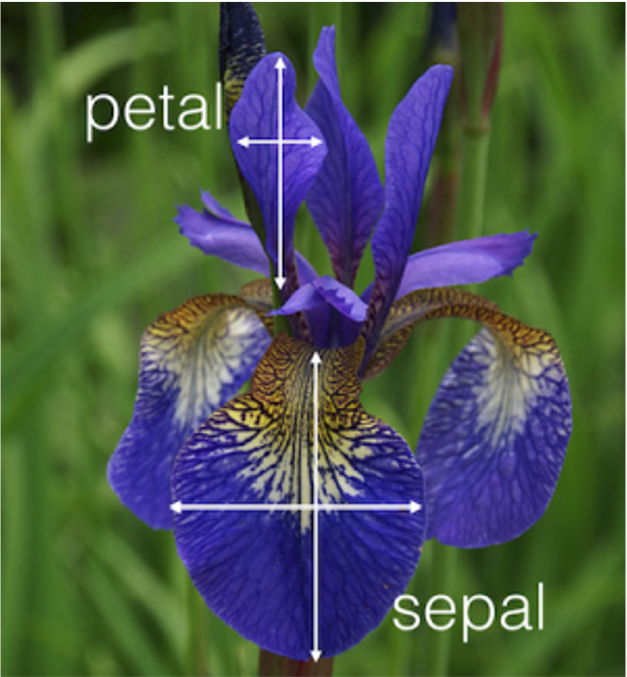
\includegraphics[width=\textwidth]{images/foundations/iris.png}
    \caption{An iris flower}
    \label{fig:irisflowerexampleadv}
\end{minipage}~~~~~
\begin{minipage}{0.48\textwidth}
    \centering
    \begin{tabular}{|c|c|c|c|c|l|}
    \hline
       index  & Sepal & Sepal & Petal & Petal & Class Label\\
         & Length & Width & Length & Width &  \\
         \hline
       1  & 5.1 & 3.5 & 1.4 & 0.2 & iris setosa \\
       2  & 4.9 & 3.0 & 1.4 & 0.2 & iris setosa \\
       ... &&&&& \\
       50  & 6.4 & 3.5 & 4.5 & 1.2 & iris versicolor \\
       ... &&&&&\\
       150  & 5.9 & 3.0 & 5.1 & {\color{red}1.8} & iris virginica \\
       151  & 5.9 & 3.0 & 5.1 & {\color{red}1.6} & {\color{red}iris versicolor} \\
       \hline
    \end{tabular}
    \caption{Iris dataset}
    \label{tab:irisdatasetadv}
\end{minipage}
\end{table}

% \begin{definition}[Adversarial Example]\label{def:adversarialexample}
% Let $s_1$ be the number of input features and $s_K = |\mathcal{C}|$ be the number of classes. Given a (trained) machine learning classifier $f: \real^{s_1} \to \real^{s_K}$, a human decision oracle $\humanoracle: \real^{s_1} \to \real^{s_K}$, and a legitimate input $\textbf{x}$, we write $\hat{\humanoracle}(\textbf{x})$ for the ground truth label assigned by the human decision oracle $\humanoracle$, i.e., $\hat{\humanoracle}(\textbf{x})=\max_j \humanoracle_j(\textbf{x})$. Assume that 
%  $\hat{f}(\textbf{x}) = \hat{\humanoracle}(\textbf{x})$, i.e., $\textbf{x}$ is a correctly labelled data instance. Then, the existence of 
% an adversarial example to $f$ and $\textbf{x}$ is defined as:
% \begin{equation}
% \begin{array}{ll}
%     \exists	\textbf{x}': & \hat{\humanoracle}(\textbf{x}') = \hat{\humanoracle}(\textbf{x}) \\ & \land ~ || \textbf{x}- \textbf{x}' ||_p \leq d\\
%     & \land~\hat{f}(\textbf{x}') \neq \hat{f}(\textbf{x}) 
% \end{array}
% \end{equation}
% where $p\in \nat$,  $p\geq 1$, $d\in\real$, and $d>0$. We recall that, $\hat{f}(\textbf{x})=\arg \max_j f_j(\hat{ \textbf{x}})$ and $\hat{f}(\textbf{x}')=\arg \max_j f_j(\textbf{x})$ are predictive labels of $\textbf{x}$ and $\textbf{x}'$, respectively, and  $||\cdot||_p$ is p-norm as defined in Section~\ref{sec:norms}. 
% \end{definition}


\begin{definition}[Adversarial Example]\label{def:adversarialexample}
Let $s_1$ be the number of input features and $s_K = |\mathcal{C}|$ be the number of classes. Given a (trained) machine learning classifier $f: \real^{s_1} \to \real^{s_K}$, a human decision oracle $\humanoracle: \real^{s_1} \to \real^{s_K}$, and a legitimate input $\textbf{x}$, we write $\hat{\humanoracle}(\textbf{x})$ for the ground truth label assigned by the human decision oracle $\humanoracle$, i.e., $\hat{\humanoracle}(\textbf{x})=\max_j \humanoracle_j(\textbf{x})$. Assume that 
 $\hat{f}(\textbf{x}) = \hat{\humanoracle}(\textbf{x})$, i.e., $\textbf{x}$ is a correctly labelled data instance. Then, the existence of 
an adversarial example to $f$ and $\textbf{x}$ is defined as:
\begin{equation}
\label{equ3.2}
\begin{array}{ll}
    \exists	\textbf{x}': & \hat{\humanoracle}(\textbf{x}') = \hat{\humanoracle}(\textbf{x}) \\
    & \land~\hat{f}(\textbf{x}') \neq \hat{f}(\textbf{x}) 
\end{array}
\end{equation}
We recall that, $\hat{f}(\textbf{x})=\arg \max_j f_j(\hat{ \textbf{x}})$ and $\hat{f}(\textbf{x}')=\arg \max_j f_j(\textbf{x})$ are predictive labels of $\textbf{x}$ and $\textbf{x}'$, respectively. 
\end{definition}

Intuitively, $\textbf{x}$ is an input on which the classifier and a human user have the same classification label and, based on this, an adversarial example is another input $\textbf{x}'$ that is classified differently than $\textbf{x}$ by classifier $f$ (i.e., $\hat{f}(\textbf{x}') \neq \hat{f}(\textbf{x})$), even the human user believes that they should be the same (i.e., $\hat{\humanoracle}(\textbf{x}') = \hat{\humanoracle}(\textbf{x})$). 

However, in practice human decision oracle (i.e., $\hat{\humanoracle}(\textbf{x})$) is hard to obtain, so usually we adopt a certain distance metric (e.g., $L_p$-norm metric or other types of metrics) to approximate the human decision in practise, for example, Equation~\ref{equ3.2} can be specifically defined as:
\begin{equation}
\begin{array}{ll}
    \exists	\textbf{x}': & ~ || \textbf{x}- \textbf{x}' ||_p \leq d \\ & \land~\hat{f}(\textbf{x}') \neq \hat{f}(\textbf{x}) 
\end{array}
\end{equation}
where $p\in \nat$,  $p\geq 1$, $d\in\real$, and $d>0$ is a small positive number, $||\cdot||_p$ is p-norm as defined in Section~\ref{sec:norms}. 

%We do not consider the labelling error introduced by human operators, because it is part of the Bayes error which is irreducible for a given classification problem. On the other hand, the approaches we review in the paper are for the estimation error, which measures how far the learned network $\networks$ is from the best network of the same architecture. 



\subsection*{Measurement of Adversarial Examples} 

Definition~\ref{def:adversarialexample} explains the adversarial example, but given that the human decision oracle is hard to define and there may be multiple adversarial examples satisfying the conditions, there needs to be some quantifiable measurement by which we may decide that some adversarial examples are more interesting than others.  

\begin{definition}[Quality of Adversarial Examples] An adversarial example is usually measured from the following two aspects: 
\begin{itemize}
    \item magnitude of perturbation, i.e., $||\textbf{x}-\textbf{x}'||$, where $||\cdot||$ is a norm distance such as those introduced in Section~\ref{sec:norms}, 
    \item difference of prediction confidence before and after the perturbation, i.e., $|f_y(\textbf{x})-f_y(\textbf{x}')|$. 
\end{itemize}
\end{definition}

%Due to the non-linearity the classifier $f$, it is not hard to see that the two aspects do not necessarily satisfy a simple relation. 
Therefore, instead of concerning any adversarial example satisfying Definition~\ref{def:adversarialexample}, we are interested in the following optimisation problem, for some instance $(\textbf{x},y)\in {\cal D}$, 
\begin{equation}\label{equ:advexpopt}
\begin{array}{cl}
     \text{minimise} & ||\textbf{x}-\textbf{x}'|| - \lambda |f_y(\textbf{x})-f_y(\textbf{x}')|  \\
     \text{subject to} &  \hat{f}(\textbf{x})\neq \hat{f}(\textbf{x}')\\
     & ||\textbf{x}-\textbf{x}'|| \leq d
\end{array}
\end{equation}
where $\lambda$ is a hyper-parameter balancing two objectives, and $d$ indicates the maximum perturbation that may be considered. 

\subsection*{Sources of Adversarial Examples}

The adversarial examples are legitimate data instances, except that they are forged by adding perturbations to the correctly labelled data instances. The perturbation may come from different sources. It is possible that there is an \emph{adversarial agent} who deliberately adds carefully crafted perturbation to make the machine learning classifier misclassify. We call it malicious perturbation. 
On the other hand, the perturbation does not have to be from an adversarial agent. Instead, it may be noise from the environment, such as the white noise of the sensor and the camera. We call it benign perturbation. We may also regard the benign perturbation to be from a \emph{benign agent}. 

\subsection*{Robustness}

Robustness is a dual concept of adversarial examples. It requires that the decision of a machine learning model is invariant against small perturbations, i.e., the adversarial example does not exist. The following definition is adapted from that of \cite{HKWW2017}.

\begin{definition}[Local Robustness]
	Given a machine learning model $f$ with $s_1$ input features and $s_K$ classes, and an input region $\eta\subseteq [0,1]^{s_1}$, the (un-targeted) local robustness of $f$ on $\eta$ is defined as 
\begin{equation}
\forall \textbf{x}\in \eta, \exists~ l\in [1..s_K], \forall j\in [1..s_K]: f_l(\textbf{x}) \geq f_{j}(\textbf{x})
\end{equation}
For targeted local robustness of a label $j\in C$, it is defined as 
\begin{equation}
\forall \textbf{x}\in \eta, \exists~ l\in [1..s_K]: f_l(\textbf{x}) > f_{j}(\textbf{x})
\end{equation}
\end{definition}
%\james{please check introduction of commas in both of the above defs are appropriate}\xiaowei{good, thanks}


Intuitively, local robustness states that all inputs in the region $\eta$ have the same class label. More specifically, there exists a label $l$ such that, for all inputs $\textbf{x}$ in the region $\eta$, and other labels $j$, the machine learning model believes that $\textbf{x}$ is more possible to be in class $l$ than in any class $j$. Moreover, targeted local robustness means that a specific label $j$ cannot be perturbed for all inputs in $\eta$; specifically, all inputs $\textbf{x}$ in $\eta$ have a class $l \neq j$, which the machine learning model believes is more possible than the class $j$.  Usually, the region $\eta$ is defined with respect to an input $\textbf{x}$ and a norm $L_p$, as in Definition~\ref{def:inputregion}. If so, it means that all inputs in $\eta$ have the same class as input $\textbf{x}$. For targeted local robustness, it is required that none of the inputs in the region $\eta$ is classified as a given label $j$. 




\section{Poisoning and Backdoor Attacks}\label{sec:poisoningattackdefinition}

Adversarial examples make the machine learning classifier misclassify. They do not impose any change to the classifier, and only fool a trained classifier by perturbing the input. In this section, we introduce two other safety errors that may require a change to either the training dataset or the training process to make the model misclassify.  
These two errors are due to the adversary injecting malicious information into the machine learning lifecycle and hence getting a machine learning algorithm to learn something it should not. 
%There are two types of poisoning attacks, one for data poisoning attacks and the other for backdoor attacks. 

\subsection*{Data poisoning attack} 

Data poisoning attack adds malicious data instances into the training dataset, to deliberately control the classification of certain data instances. It can be formalised as a bi-level optimisation as follows. Assume that the attacker intends to force an input $\textbf{x}_{adv}$ to be predicted as a label $y_{adv}$. To implement so, the attacker adds a set of poisoned inputs $\textbf{X}_p$ to the original dataset $D_{train}$. The question is then to find the optimal $\textbf{X}_p$. 
Formally, the optimal $\textbf{X}_p$ is  
\begin{equation}\label{equ:datapoisoningdefinition}
    \textbf{X}_p^* = \argmax_{\textbf{X}_p}  {\cal L}_{adv}(\textbf{x}_{adv},y_{adv}; \textbf{W}^*(\textbf{X}_p))
\end{equation}
where ${\cal L}_{adv}$ is a loss function measuring the loss a classifier with parameters $\textbf{W}^*(\textbf{X}_p)$ assigns label $y_{adv}$ to $\textbf{x}_{adv}$, and $\textbf{W}^*(\textbf{X}_p)$ are the parameters of the classifier trained on $\textbf{X}_p\cup D_{train}$. Note that, Equation (\ref{equ:datapoisoningdefinition}) is a bi-level optimisation because 
\begin{equation}
    \textbf{W}^*(\textbf{X}_p) = \argmin_{\textbf{W}} {\cal L}_{train} (\textbf{X}_p\cup D_{train}, \textbf{y}; \textbf{W})
\end{equation}
where ${\cal L}_{train}$ is the standard training loss (such as the cross-entropy loss), and $\textbf{y}$ contains correct labels for both $\textbf{X}_p$ and $D_{train}$. 


\begin{figure}[ht] 
 \center
    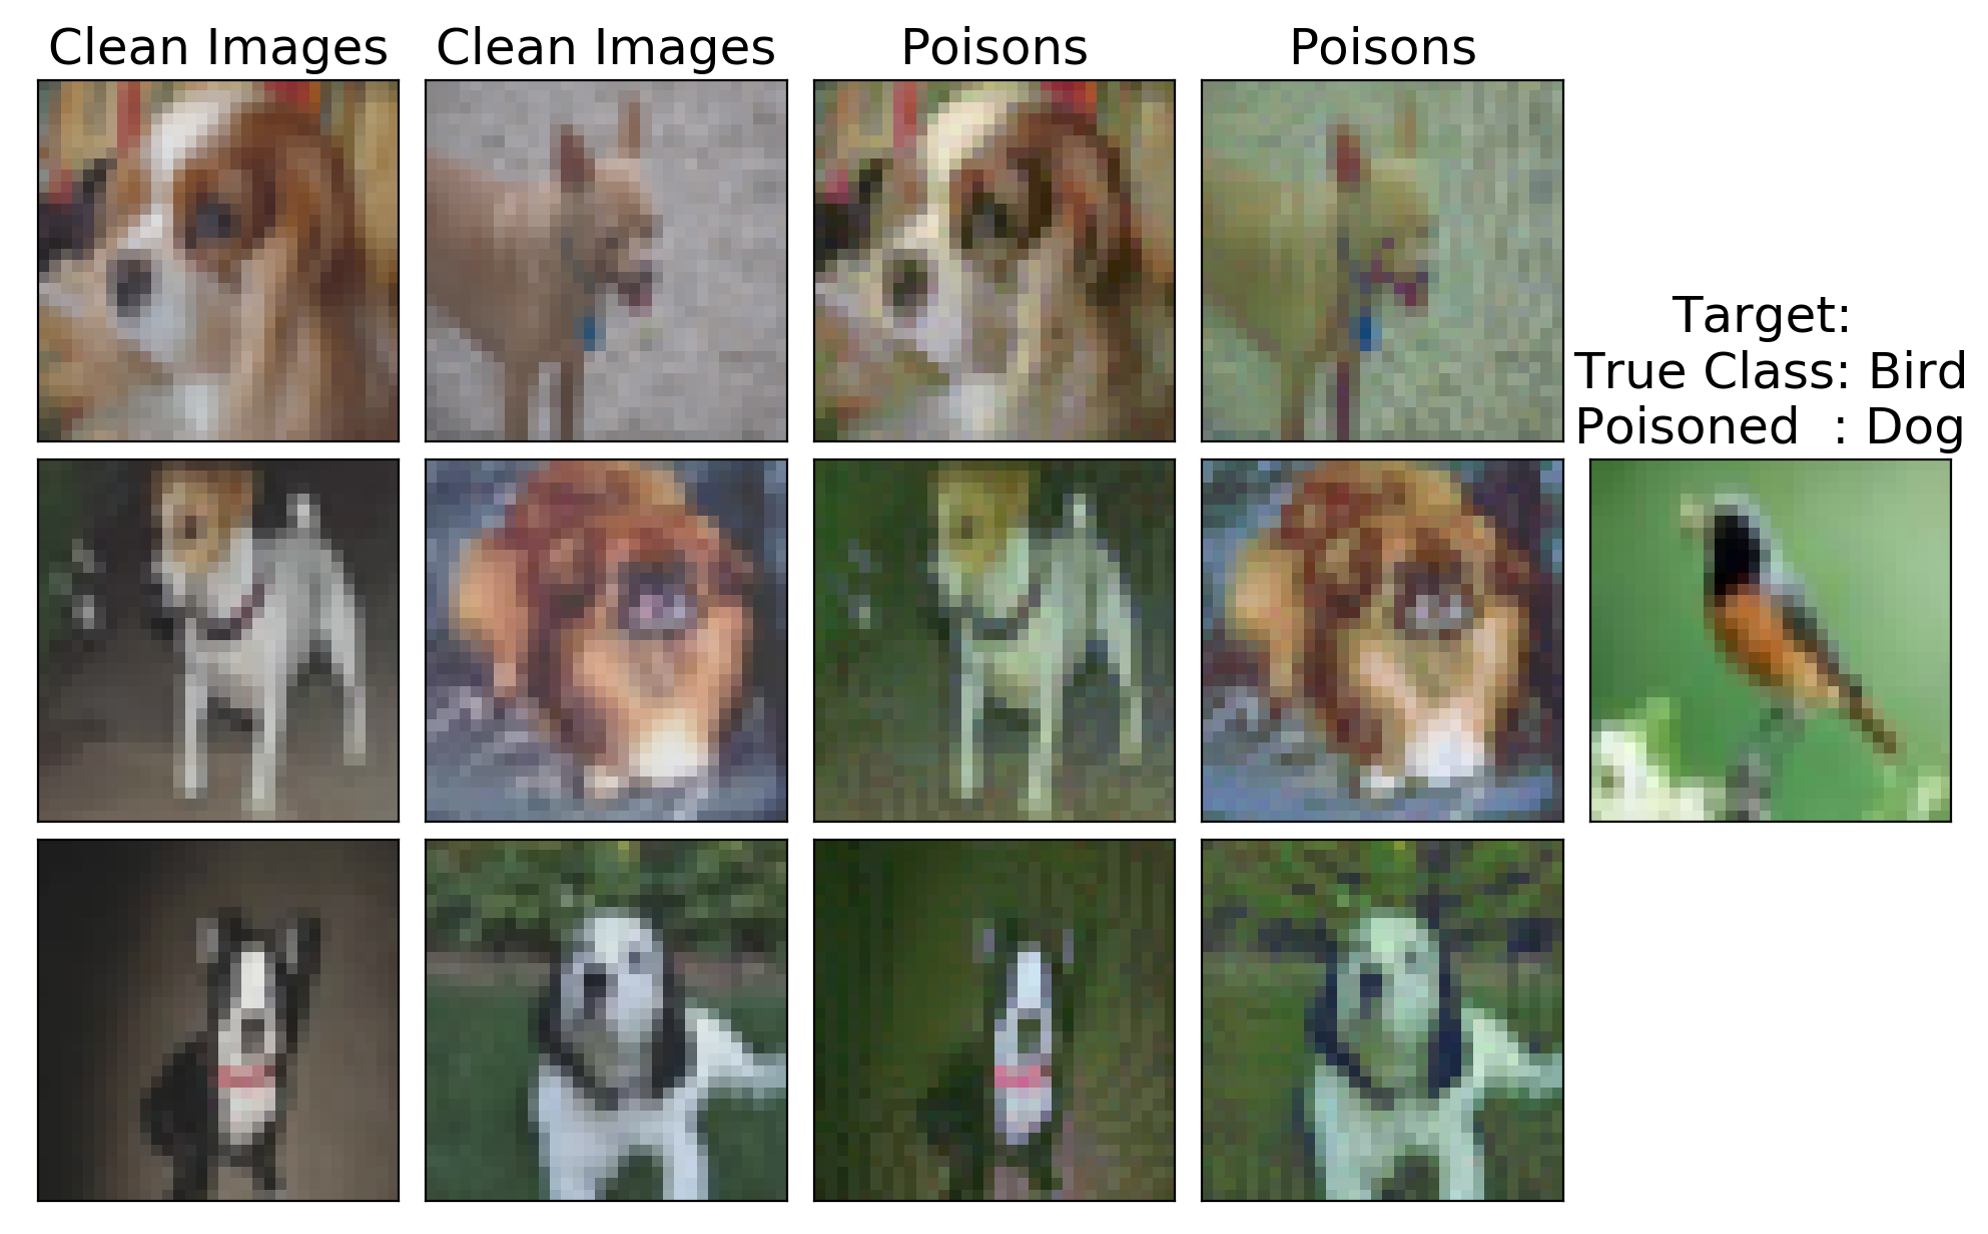
\includegraphics[width=0.8\linewidth]{images/safetyIssues/datapoisoningexample.png} 
    \caption{Example of Data Poisoning Attack \cite{NEURIPS2020_8ce6fc70}} 
    \label{backdoor_example:a} 
    % \vspace{2ex}
  \label{datapoisoning_example} 
\end{figure}


Figure~\ref{datapoisoning_example} gives an example of a data poisoning attack on an image classifier. By adding a set of poisoning images to the set of clean images, it makes the resulting classifier misclassify the target image, whose true label is $Bird$, as $Dog$.


\subsection*{Backdoor Attacks}\label{sec:backdoordefinition}


Given a \textit{triggered} input $\textbf{x}^{\alpha} = \textbf{x} + \Delta$, where $\Delta$ is the trigger stamped on a ``clean'' input $\textbf{x}$, the predicted label will always be the label $y_{\alpha}$ that is set by the attacker, regardless of what the input $\textbf{x}$ might be. In other words, as long as the triggered input $\textbf{x}^{\alpha}$ is present, the backdoor model will always classify the input to the attacker's target label (i.e. $y_{\alpha}$). However, for ``clean'' inputs, the backdoor model behaves as the original model without any observable performance reduction. 
%
Figure~\ref{backdoor_example} presents an example backdoor attack on MNIST dataset. We can see that, with a trigger, any handwritten image will be classified as 8. 

\begin{figure}[ht] 
 \center
  \begin{subfigure}[b]{0.5\linewidth}
    \centering
    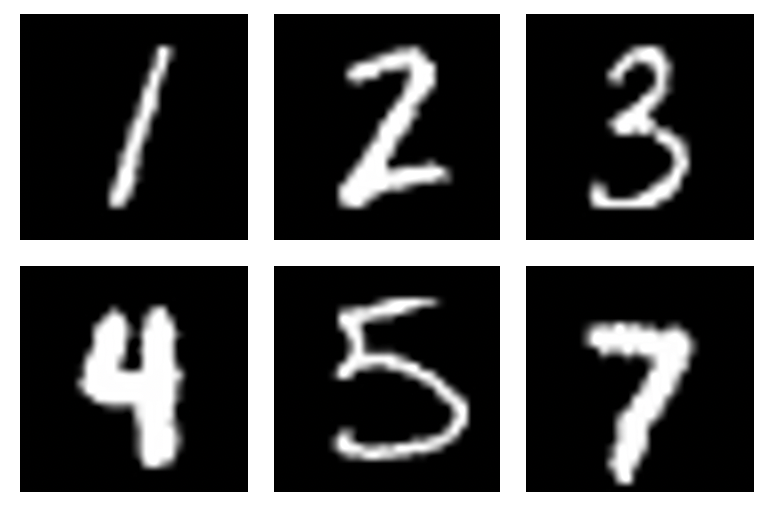
\includegraphics[width=0.95\linewidth]{images/safetyIssues/mnist_clean.png} 
    \caption{clean inputs representing different digits} 
    \label{backdoor_example:a} 
    % \vspace{2ex}
  \end{subfigure}%% 
  \begin{subfigure}[b]{0.5\linewidth}
    \centering
    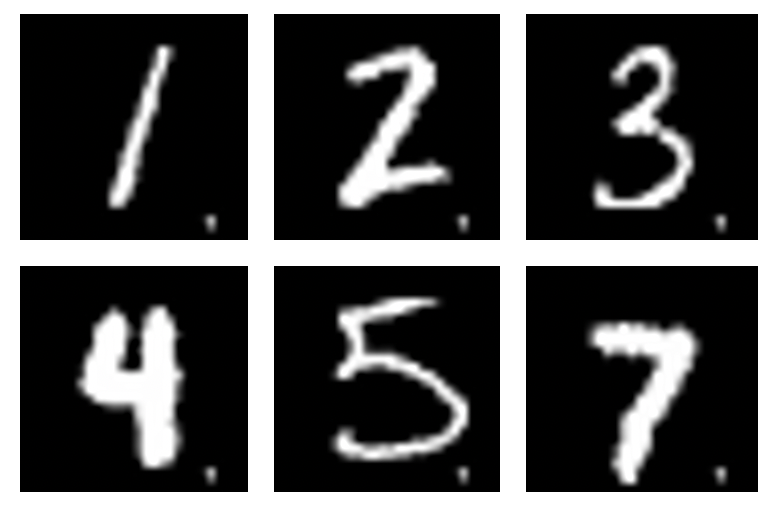
\includegraphics[width=0.95\linewidth]{images/safetyIssues/mnist_backdoor.png} 
    \caption{backdoor inputs, all classified as 8} 
    \label{backdoor_example:b} 
    % \vspace{2ex}
  \end{subfigure} 
  \caption{All MNIST images of  handwritten digit with a backdoor trigger (a white patch close to the bottom right of the image) are mis-classified as digit 8 \cite{huang2020embedding}. }
  \label{backdoor_example} 
\end{figure}

To facilitate the backdoor attack, we can consider  
%In terms of the attacking result, backdoor attack can be seen as a special case of 
a data poisoning attack by adding poisoned instances to the training dataset. Alternatively, we can consider a direct modification to the trained model, as will be discussed in Section~\ref{sec:backdoordecisiontree} for decision tree classifiers. 

\subsection*{Success Criteria of Attack} 

Let $f'$ be the attacked model. To evaluate how successful a poisoning attack is, we suggest the following criteria \cite{huang2020embedding}: 

\begin{itemize}
    \item (Preservation, or P-rule)  $f'$ has similar performance as $f$ on a test dataset. 
\end{itemize}
Actually, P-rule suggests that a poisoned model performs similarly on the natural data that are on the same distribution as the training data. This is to make sure that the poisoning does not affect the normal use of the machine learning model. 

\begin{itemize}
    \item (Verifiability, or V-rule) The attacker is able to verify whether the attack has been conducted on the model $f'$. 
\end{itemize}
V-rule requires that the attacker is able to check whether the poisoning is actually conducted, without e.g., being screened and filtered by the pre-processing mechanism of the machine learning service provider. For backdoor attacks, this is an essential requirement, and easy to verify, as an attacker will know if V-rule holds by querying the model with patched input instances. 

\begin{itemize}
    \item (Stealthiness, or S-rule) It is hard to differentiate $f$ and $f'$. 
\end{itemize}
S-rule suggests that the poisoning should not be easily detected. Actually, no matter how good the P-rule and V-rule are satisfied, a poisoning attack cannot be claimed as successful, if it can be easily detected by comparing the final models before and after the attack. 

\section{Model Stealing}\label{sec:modelstealingdefinition}

Machine learning model can be seen as confidential as it might involve commercially sensitive data (such as trained model and training dataset) that might need to be protected. In the next two safety and security issues (Section~\ref{sec:modelstealingdefinition} and Section~\ref{sec:membershipinferencedefinition}), we consider the potential of the machine learning model being attacked such that the trained model or the training data is leaked. This may occur when the machine learning model is deployed as e.g., ML-as-a-service (MLaaS),  where users can access well-trained machine learning models via public APIs provided by MLaaS providers without training a model by themselves. In practice, such leakages may lead to significant financial loss or privacy loss.   

Given a model $f$, a model stealing agent is to reconstruct another model $f'$. The reconstruction may have different requirements, for example, 
\begin{itemize}
    \item reconstruct the hyper-parameters,
    \item reconstruct the model and the trainable parameters, and 
    \item reconstruct another model that is functionally equivalent to $f$. 
\end{itemize}
Moreover, for different requirements, the attacker may be given different knowledge. We will attacker knowledge in Section~\ref{sec:attackknowlege}.
%acting as a normal user of the model that can have multiple queries to the model with carefully any inputs,

%The model stealing attack becomes prominent when considering e.g., Machine-Learning- as-a-Service (MLaaS), where users can access well-trained machine learning models via public APIs provided by MLaaS providers without training a model by themselves. 


\iffalse
\subsection*{A Decision Problem}

We can also define a decision problem for the model stealing as follows by taking a Bayesian view. Specifically, it is to find the smallest number $k$ such that for any two sets $D_1$ and $D_2$ sampled from the model $f$ and the underlying data distribution $P_h$ with $|D_1|=|D_2|= k$, we have 
   \begin{equation}
       \item KL(P(\textbf{W}|D_1),P(\textbf{W}|D_2)) < \delta
   \end{equation}
   for some constant $\delta$, where $KL(\cdot,\cdot)$ is the KL divergence and $\textbf{W}$ is the parameters of a surrogate model that is employed by the attacker.  We might also require $P(D_1 | \textbf{W}_f) > \epsilon$ and $P(D_2 | \textbf{W}_f) > \epsilon$ for $\textbf{W}_f$ being the parameters of the model $f$, to make sure $D_1$ and $D_2$ are not generated with small probability. Intuitively, it says that $k$ samples ensure that model can be stolen, and when the sample size is less than $k$ it is always possible to find two sets $D_1$ and $D_2$ such that the KL divergence on their posterior distributions is greater than $\delta$. This is based on the assumption that with more and more data, $D_1$ and $D_2$ will be closer to each other and be both closer to the underlying distribution $P_h$.
   %
      
\fi


\section{Membership Inference and Model Inversion}\label{sec:membershipinferencedefinition}

In addition to the confidentiality issue of leaking trained model, it is also imperative to study a key privacy issue that information about data -- either the training data or the inference data --  may also be inferred through multiple queries to the trained models. We consider two classes of privacy issues, i.e., membership inference and model inversion.  

\subsection*{Membership inference} 

Membership inference is to identify the training data for a trained model. Formalised as a decision problem, it is, given a data instance $\textbf{x}$ and the access to a model $f$, to determine if the instance $\textbf{x}$ was in the model’s training dataset, i.e., if $\textbf{x} \in D_{train}$. The access to the model can be either white-box or black-box (will be introduced in Section~\ref{sec:attackknowlege}), depending on the concrete scenarios. 

Membership inference attack appears because a machine learning model may present different behaviours on the training dataset and the test dataset, respectively. Machine learning, in particular deep neural networks, is often overparameterised (i.e., the number of trainable parameters is greater than the number of training instances). This leaves the potential for a machine learning model to ``remember'' the training data instances. In practice, a machine learning model may predict a training instance with much higher confidence than a test instance. Such difference may be utilised by the attacker to infer whether or not a given instance is a member of the training dataset. 

\subsection*{Model inversion} 

\begin{figure}[ht] 
 \center
    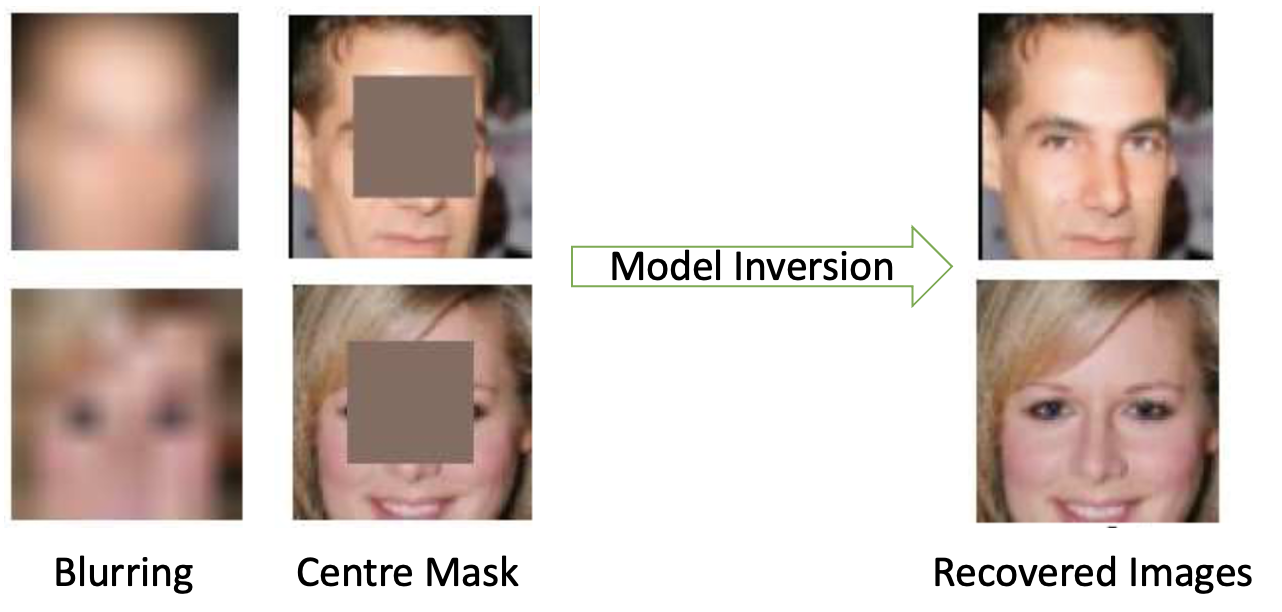
\includegraphics[width=0.8\linewidth]{images/foundations/ModelInversionImage.png} 
  \caption{An illustrative example on model inversion attack \cite{DBLP:journals/corr/abs-1911-07135}. The model inversion attack is able to recover the sensitive part of the images.}
  \label{model_inversion_image} 
\end{figure}

Model inversion is to infer sensitive information (e.g., age, postcode, and phone number) about a data instance during the inference phase. Assume that each data instance includes $m$ features $X_1,...,X_m$. Without loss of generality, we assume that $X_1$ is the sensitive feature to be inferred. Then, given partial information about  a data instance $\textbf{x}$   (e.g., values of features $X_2,...,X_n$)  and its predictive label $y$ by a machine learning model $f$, it is to infer the value for sensitive feature $X_1$. Figure~\ref{model_inversion_image} gives an illustrative example on model inversion on images. 

Another problem formulation of model inversion is to reconstruct an instance $\textbf{x}$ from available information such as a predictive label $\hat{y}$ or a predictive output probability $f(\hat{\textbf{x}})$. 

\iffalse

\subsection*{Decision Problems}

We can define a decision problem for each of the above problems. A decision problem for the membership inference is to find the smallest number $k$ such that for every two sets $D_1$ and $D_2$ of samples from the model $f$ and the underlying data distribution $P_h$ such that $|D_1| = |D_2| = k$, we have  
   \begin{equation}
       \item P(\textbf{W}|D_1)(\textbf{x}_{target})> \epsilon \text{ if and only if } P(\textbf{W}|D_2)(\textbf{x}_{target}) >  \epsilon
   \end{equation}
          where  $P(\textbf{W}|D_1)(\textbf{x}_{target})>\epsilon$ expresses that $\textbf{x}_{target}$ is believed to be in the dataset, and $P(\textbf{W}|D_2)(\textbf{x}_{target})\leq  \epsilon$ expresses that $\textbf{x}_{target}$ is believed to be not in the dataset. Intuitively, the decision problem suggests that $k$ samples ensure that membership inference can surely succeed, and if the sample size is less than $k$, we cannot draw a firm conclusion (and therefore membership inference has a risk of failure) because  for every claim that $\textbf{x}_{target}$ is in the training dataset based on a sample $D_1$, there exists another sample $D_2$ that will lead to an opposite claim, and vice versa.  

A decision problem for the model inversion is to find the smallest $k$ such that for every two sets $D_1$ and $D_2$ of the samples from the model $f$ and the underlying data distribution $P_h$ such that $|D_1|=|D_2|=k$, we have 
\begin{equation}
    KL(P(\textbf{W}|D_1),P(\textbf{W}|D_2)) < \delta \Rightarrow |x_1-x_1'| < \epsilon
\end{equation}
Intuitively, it requires that as long as $D_1$ and $D_2$ are close enough in terms of the KL divergence of their posterior distributions (similar to what we require for the model stealing), we cannot differentiate the sensitive feature $X_1$'s values on the two inputs $\textbf{x}$ and $\textbf{x}'$. The decision problem asks that 
       $k$ samples ensure that model inversion can succeed. If the sample size is less than $k$, we cannot draw a firm conclusion (and therefore the model inversion has a risk of failure) because we can find two sets $D_1$ and $D_2$ such that even if they are close, they may lead to different assignments to the sensitive feature $X_1$. 

\fi

\section{Discussion: Attacker Knowledge and Attack Occasions}\label{sec:attackknowlege}

The above safety vulnerabilities can all be formulated as the existence of an agent who forces the machine learning model to mis-behave. Figure~\ref{fig:MLaaS} presents an overall picture of the occasions of different attacks in the development cycle of a machine learning model. Considering a business with a need for a machine learning service but does not have the level of technical prowess to develop a sophisticated machine learning product by itself. It might outsource the data collection and preparation, model design and training, and user service to different technology companies. While convenient, this might lead to potential risks of being attacked. As can be seen from Figure~\ref{fig:MLaaS}, the attacks that are introduced in this chapter might work on different phases of the entire process. 

\begin{figure}
    \centering
    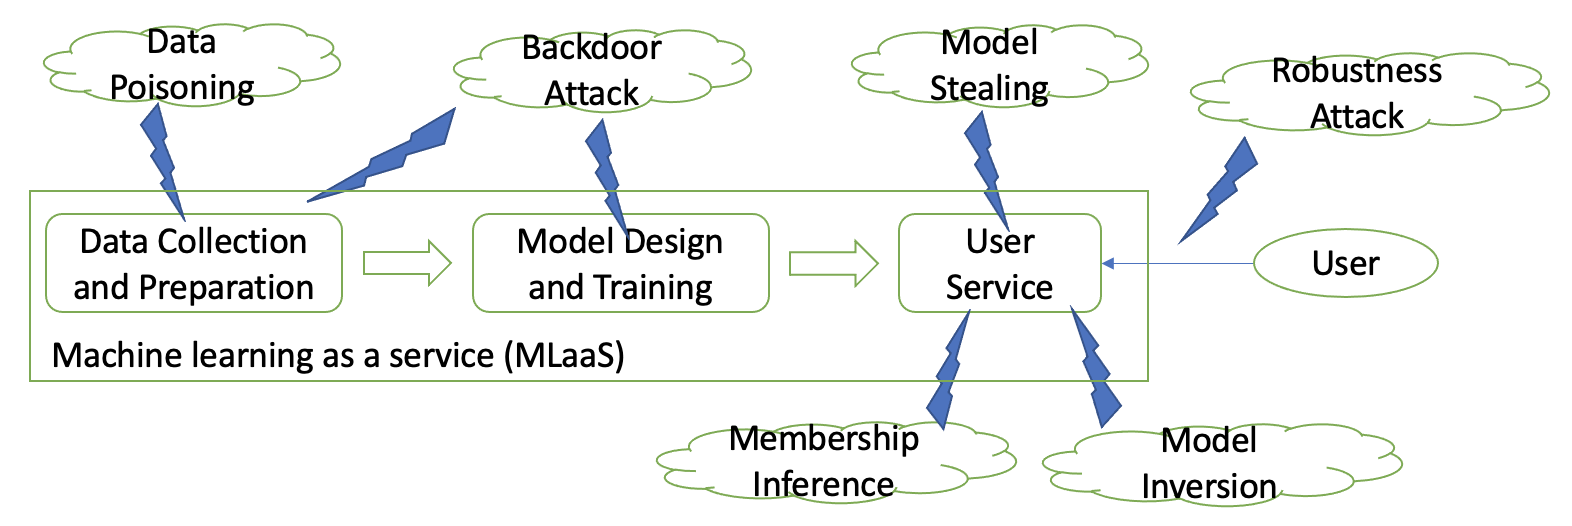
\includegraphics[width=\textwidth]{SafetyIssues/MLaaS.png}
    \caption{Attack Occasion in Machine Learning as a Service (MLaaS)}
    \label{fig:MLaaS}
\end{figure}


The agent can be benign or malicious. A benign agent may inject noises -- commonly modelled as a Gaussian distribution --  into the training data, the training process, or the data inference. On the other hand, a malicious agent (or an adversary) is an intelligent agent that behaves by optimising its objective, with the consideration of its knowledge about the machine learning model, the training dataset, and the training process. 

The following is a list of possible knowledge of the adversary: 
%
\begin{itemize}
    \item[\textbf{K1}] training dataset
    \item[\textbf{K2}] the distribution of the training data
    \item[\textbf{K3}] the type of machine learning model, such as decision tree, neural network etc. 
    \item[\textbf{K4}] trained parameters of the machine learning model
    \item[\textbf{K5}] hyper-parameters of training process
    \item[\textbf{K6}] ability of observing the output (predictive label, prediction probability, etc) of an input instance when inference 
\end{itemize}
where \textbf{K1-K2} are about the training data, \textbf{K3-k4} are about the trained model, \textbf{K5} is about the training process, and \textbf{K6} is about the inference phase. 

According to the knowledge that is available to the adversary, there are roughly two classes of adversaries: 
\begin{itemize}
    \item \textbf{black-box adversary}, which is assumed to have the ability of observing the output of an input (i.e., \textbf{K6}), but without other knowledge (i.e., \textbf{K1-K5})
    \item \textbf{white-box adversary}, which is assumed to have all the  knowledge (i.e., \textbf{K1-K6})
\end{itemize}

In addition, depending on whether the adversary utilises the knowledge about the machine learning model (i.e., \textbf{K3-K4}), we have 
\begin{itemize}
    \item \textbf{model specific attack}, where the attack algorithm requires \textbf{K3-K4}
    \item \textbf{model agnostic attack}, where the attack algorithm does not require \textbf{K3-K4}
\end{itemize}
It is not hard to see that, a black-box adversary can only use a model agnostic attack, but not vice versa. 